\documentclass[aspectratio=169]{beamer}
% \usepackage[utf8]{inputenc}
\usetheme{metropolis}
\usecolortheme{orchid}
\usepackage{amsmath}
\usepackage{amssymb}
\usepackage{amsthm}
\usepackage{multirow}
\usepackage[ruled]{algorithm2e}
\usepackage{mathtools}
\usepackage{caption}
\usepackage{epstopdf}
\usepackage{hyperref}
\setbeamerfont{footnote}{size=\tiny}

\usepackage{tikz}
\usetikzlibrary{mindmap,shadows,tikzmark,positioning,arrows.meta}

% Information boxes
\newcommand*{\info}[4][16.3]{%
  \node [ annotation, #3, scale=0.65, text width = #1em,
          inner sep = 2mm ] at (#2) {%
  \list{$\bullet$}{\topsep=0pt\itemsep=0pt\parsep=0pt
    \parskip=0pt\labelwidth=8pt\leftmargin=8pt
    \itemindent=0pt\labelsep=2pt}%
    #4
  \endlist
  };
}

\tikzset{%
  >={Latex[width=2mm,length=2mm]},
  % Specifications for style of nodes:
            base/.style = {rectangle, rounded corners, draw=black,
                           minimum width=4cm, minimum height=1cm,
                           text centered, font=\sffamily},
  activityStarts/.style = {base, fill=blue!30},
       startstop/.style = {base, fill=red!30},
    activityRuns/.style = {base, fill=green!30},
         process/.style = {base, minimum width=2.5cm, fill=orange!15,
                           font=\ttfamily},
}
\renewcommand\textbullet{\ensuremath{\bullet}}
\newcommand\scalemath[2]{\scalebox{#1}{\mbox{\ensuremath{\displaystyle #2}}}}
\newcommand{\norm}[1]{\left\lVert#1\right\rVert}

%%% Bibliography
\usepackage[citestyle=numeric,style=numeric,backend=biber,doi=false,isbn=false,url=false]{biblatex}
\addbibresource{references.bib}

%%% Suppress biblatex annoying warning
\usepackage{silence}
\WarningFilter{biblatex}{Patching footnotes failed}

%%% new theorems %%%%%%%%%%%%%%%%%%%%%%%%%%%%%%%%%%%%%%%%%%%%%%%%%%%%%%%%%%%%%%
\theoremstyle{definition}
\newtheorem{mydef}{Definition}

\theoremstyle{plain}
\newtheorem{mylemma}{Lemma}[section]
\newtheorem{mytheorem}{Theorem}[section]
\newtheorem{myproposition}{Proposition}[section]
\newtheorem{myproblem}{Problem}[section]
\newtheorem{mydefinition}{Definition}[section]
\newtheorem{myassumption}{Assumption}[section]

\theoremstyle{remark}
\newtheorem{myremark}{Remark}[section]

\newcounter{saveenumi}
\newcommand{\seti}{\setcounter{saveenumi}{\value{enumi}}}
\newcommand{\conti}{\setcounter{enumi}{\value{saveenumi}}}

\resetcounteronoverlays{saveenumi}

\title{Controles}
\subtitle{\small Clase 4: Sintonización de Controladores}
\author{Gerardo Becerra, Ph.D.}
\institute{Pontificia Universidad Javeriana\\ Departamento de Electrónica}
\date{Febrero 19, 2020}

\begin{document}

\frame{\titlepage}	

% \frame{\tableofcontents}

% \section{Tipos de Control}
\begin{frame}[<+->]\frametitle{Introducción}
\vspace*{5mm}
\centering
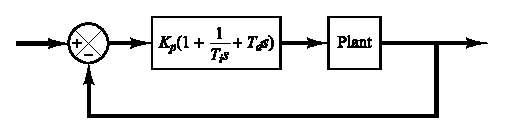
\includegraphics[width=8cm]{images/PIDController.eps}
\begin{itemize}
	\item Controlador PID $\rightarrow$ Depende de los parámetros $K_p$, $T_i$, $T_d$.
	\item \textbf{Sintonización:} Selección de valores numéricos para los parámetros, con base en algún criterio.
	\item Existen muchos criterios para sintonización de controladores.
	\begin{itemize}
		\item Experimentales
		\item Análisis de la función de transferencia
		\item Técnicas de optimización
		\item Lugar geométrico de las raíces
		\item Compensación en frecuencia
	\end{itemize}
\end{itemize}
\end{frame}

\section{Criterios Clásicos de Sintonización}
\subsection{Método de Ziegler-Nichols}
\begin{frame}[<+->]\frametitle{Método de Ziegler-Nichols}
\begin{itemize}
	\item Método experimental.
	\item Útil cuando no se conoce un modelo matemático detallado de la planta.
	\item Está diseñado para proveer un buen rechazo a perturbaciones.
	\item Produce un sobrepico grande.
	\item Los parámetros resultantes no necesariamente son óptimos. Se toman como punto de partida para un ajuste fino.
	\item Dos métodos
	\begin{enumerate}
		\item Lazo abierto: Características de la curva de reacción ante entrada paso.
		\item Lazo cerrado: Aumentar la ganancia proporcional hasta un valor crítico.
	\end{enumerate}
\end{itemize}
\end{frame}

\begin{frame}[<+->]\frametitle{Método de Ziegler-Nichols / Método 1: Lazo Abierto}
\small
\vspace*{-2mm}
\begin{columns}
\begin{column}{0.5\textwidth}
\begin{itemize}
	\item Aplicar entrada paso unitaria al sistema y medir la respuesta (experimental o simulación).
	\item Si la respuesta tiene forma de $S$, se puede aplicar el método.
	\item Caracterizar la curva obtenida usando dos parámetros: tiempo muerto $L$ y constante de tiempo $T$.
	\item Los parámetros se encuentran dibujando una recta tangente al punto de inflexión de la curva en forma de $S$.
\end{itemize}
\end{column}	
\begin{column}{0.5\textwidth}
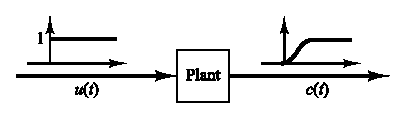
\includegraphics[width=6.5cm]{images/zieglerNichols1a.eps}\\
\vspace*{5mm}
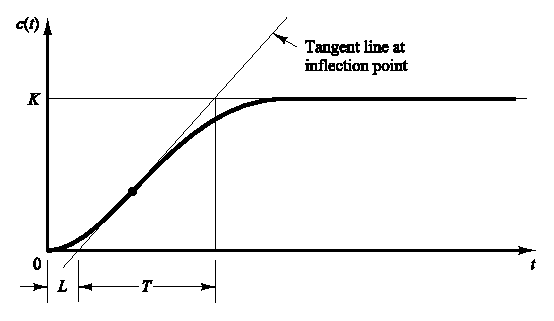
\includegraphics[width=6.5cm]{images/zieglerNichols1b.eps}
\end{column}	
\end{columns}
\end{frame}

\begin{frame}[<+->]\frametitle{Método de Ziegler-Nichols / Método 1: Lazo Abierto}
\begin{columns}
\begin{column}{0.5\textwidth}
\small
\begin{itemize}
	\item La función de transferencia $C(s)/U(s)$ se puede aproximar a un sistema de primer orden mas tiempo muerto:
	\begin{equation*}
		\frac{C(s)}{U(s)} = \frac{K e^{-Ls}}{Ts + 1}
	\end{equation*}
	\item Ziegler y Nichols sugirieron asignar los valores para los parámetros de acuerdo con la siguiente tabla:
	\begin{table}
	\begin{tabular}{c|c|c|c}
		Controlador & $K_p$ & $T_i$ & $T_d$\\
		\hline
		P   & $T/L$ & $\infty$ & 0\\
		PI  & $0.9T/L$ & $L/0.3$ & 0\\
		PID & $1.2T/L$ & $2L$ & $0.5L$
	\end{tabular}
	\end{table}
\end{itemize}
\end{column}	
\begin{column}{0.5\textwidth}
Note que el controlador PID obtenido por éste método tiene la forma:
\begin{align*}
	G_c(s) &= K_p\left( 1 + \frac{1}{T_i s} + T_d s \right)\\
	&= 1.2\frac{T}{L}\left( 1 + \frac{1}{2Ls} + 0.5 Ls \right)\\
	&= 0.6T \frac{\left( s + \frac{1}{L} \right)^2}{s}
\end{align*}
El controlador PID tiene un polo en el origen y doble cero en $s = -1/L$.
\end{column}	
\end{columns}
\end{frame}

\begin{frame}[<+->]\frametitle{Método de Ziegler-Nichols / Método 2: Lazo Cerrado}
\begin{columns}
\begin{column}{0.5\textwidth}
	\begin{itemize}
		\item Se inicia configurando $T_i = \infty$ y $T_d = 0$.
		\item Usando sólo acción proporcional, aumentar $K_p$ desde 0 hasta un valor crítico $K_{cr}$ en el cual la salida presenta oscilaciones sostenidas.
		\item Si no se obtienen oscilaciones, el método no se puede aplicar.
		\item A partir del experimento se determinan la ganancia crítica $K_{cr}$ y periodo crítico $P_{cr}$.
	\end{itemize}	
\end{column}	
\begin{column}{0.5\textwidth}
	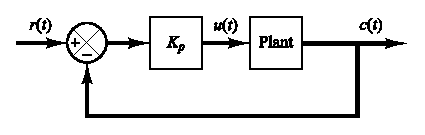
\includegraphics[width=6.5cm]{images/zieglerNichols2a.eps}\\
	\vspace*{5mm}
	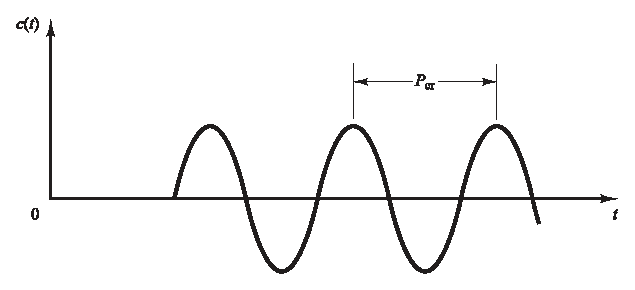
\includegraphics[width=6.5cm]{images/zieglerNichols2b.eps}
\end{column}	
\end{columns}
\end{frame}
\small
\begin{frame}[<+->]\frametitle{Método de Ziegler-Nichols / Método 2: Lazo Cerrado}
\begin{columns}
\begin{column}{0.5\textwidth}
	Ziegler y Nichols sugirieron asignar los valores para los parámetros de acuerdo con la siguiente tabla:
	\footnotesize
	\begin{table}
	\begin{tabular}{c|c|c|c}
		Controlador & $K_p$ & $T_i$ & $T_d$\\
		\hline
		P   & $0.5  K_{cr}$ & $\infty$ & 0\\
		PI  & $0.45 K_{cr}$ & $P_{cr}/1.2$ & 0\\
		PID & $0.6  K_{cr}$ & $P_{cr}/2$ & $0.125P_{cr}$
	\end{tabular}
	\end{table}
\end{column}	
\begin{column}{0.5\textwidth}
\small
Note que el controlador PID obtenido por el segundo método tiene la forma:
\begin{align*}
	G_c(s) &= K_p\left( 1 + \frac{1}{T_i s} + T_d s \right)\\
	&= 0.6 K_{cr} \left( 1 + \frac{1}{0.5 P_{cr}s} + 0.125 P_{cr}s \right)\\
	&= 0.075K_{cr}P_{cr} \frac{\left( s + \frac{4}{P_{cr}} \right)^2}{s}
\end{align*}
Entonces, el controlador PID tiene un polo en el origen y doble cero en $s = -4/P_{cr}$.
\end{column}	
\end{columns}
\end{frame}

\begin{frame}[<+->]\frametitle{Método de Ziegler-Nichols / Ejemplo}
Considere el sistema de control mostrado en la figura. Usando el método de Ziegler-Nichols, determine los parámetros del controlador PID tal que se obtenga un sobrepico máximo de aproximadamente 25\%. Si el sobrepico máximo es excesivo, realice un ajuste fino para reducirlo.
\begin{figure}
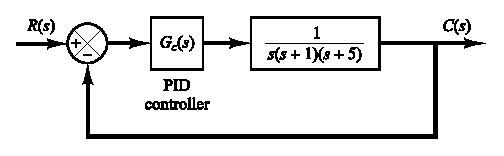
\includegraphics[width=8cm]{images/ejemplo1.eps}
\end{figure}
\end{frame}

\begin{frame}[<+->]\frametitle{Método de Ziegler-Nichols / Ejemplo}
\begin{itemize}
	\item Dado que la planta tiene un integrador, se utiliza el segundo método.
	\item Definiendo $T_i = \infty$ y $T_d = 0$, se obtiene la función de transferencia de lazo cerrado:
	\begin{equation*}
		\frac{C(s)}{R(s)} = \frac{K_p}{s(s+1)(s+5) + K_p} = \frac{K_p}{s^3 + 6s^2 + 5s + K_p}
	\end{equation*}
	\item El valor crítico de $K_p$ para obtener oscilaciones sostenidas se puede obtener usando el criterio de estabilidad de Routh-Hurwitz para el polinomio característico $q(s) = s^3 + 6s^2 + 5s + K_p = 0$:
	\begin{columns}
	\begin{column}{0.4\textwidth}
		\begin{table}
		\begin{tabular}{c|cc}
			$s^3$ & 1 & 5\\
			$s^2$ & 6 & $K_p$\\
			$s^1$ & $\frac{30-K_p}{6}$ & \\
			$s^0$ & $K_p$ & 
		\end{tabular}
		\end{table}
	\end{column}	
	\begin{column}{0.6\textwidth}
		\begin{itemize}
			\item El valor crítico de $K_p$ para obtener oscilaciones sostenidas es $K_{cr} = 30$.
			\item En éste caso, el polinomio característico es $q(s) = s^3 + 6s^2 + 5s + 30 = 0$.
		\end{itemize}
	\end{column}	
	\end{columns}
\end{itemize}
\end{frame}

\begin{frame}[<+->]\frametitle{Método de Ziegler-Nichols / Ejemplo}
\begin{columns}
\begin{column}{0.5\textwidth}
\small
\begin{itemize}
	\item Para hallar la frecuencia de la oscilación se substituye $s = j\omega$ en el polinomio característico:
	\begin{align*}
		(j\omega)^3 + 6(j\omega)^2 + 5(j\omega) + 30 = 0\\
		6(5 - \omega^2) + j\omega(5-\omega^2) = 0\\
		\Rightarrow \omega = \sqrt{5}
	\end{align*}
	\item El periodo de oscilación sostenida es:
	\begin{equation*}
		P_{cr} = \frac{2\pi}{\omega} = \frac{2\pi}{\sqrt{5}} = 2.8099
	\end{equation*}
\end{itemize}
\end{column}
\begin{column}{0.5\textwidth}
\small
\begin{itemize}
	\item Usando la tabla para el método 2, se obtienen los valores del controlador PID como:
	\begin{align*}
		K_p &= 0.6 K_{cr} = 18\\
		T_i &= 0.5 P_{cr} = 1.405\\
		T_d &= 0.125P_{cr} = 0.35124
	\end{align*}
	\item La función de transferencia del controlador PID queda:
	\begin{align*}
		G_c(s) &= 18 \left( 1 + \frac{1}{1.405s} + 0.35124 s \right)\\
		&= \frac{6.3223(s+1.4235)^2}{s}
	\end{align*}
\end{itemize}
\end{column}
\end{columns}
\end{frame}

\begin{frame}[<+->]\frametitle{Método de Ziegler-Nichols / Ejemplo}
\vspace*{5mm}
\begin{columns}
\begin{column}{0.5\textwidth}
	La respuesta del sistema en lazo cerrado ante una entrada paso es:
	\begin{figure}
		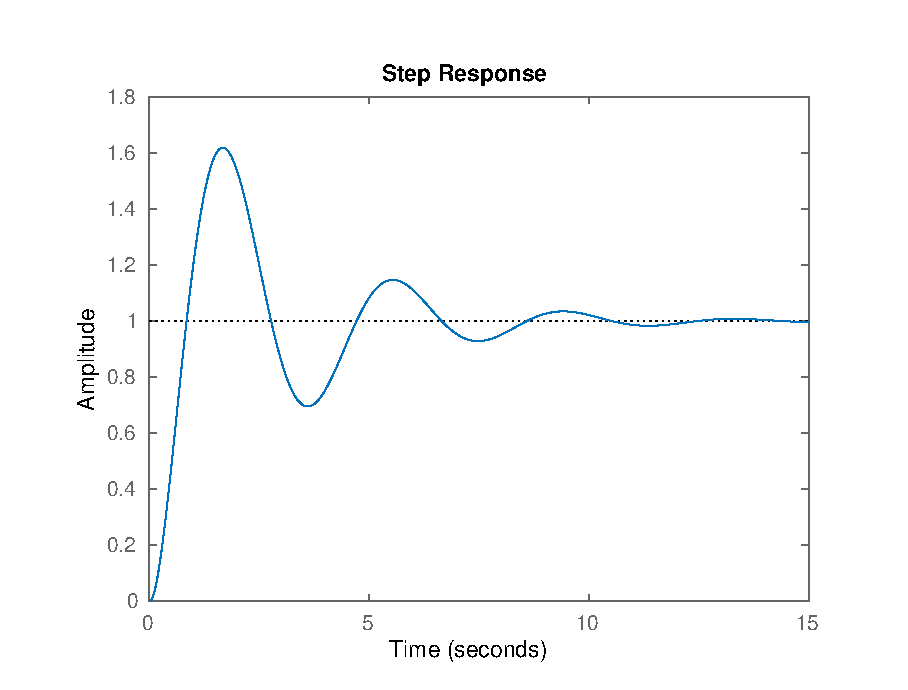
\includegraphics[width=7cm]{images/ejemplo1Respuesta.eps}
	\end{figure}
\end{column}	
\begin{column}{0.5\textwidth}
	Sobrepico 60\% approximadamente $\rightarrow$ se require ajustar los parámetros para disminuir el sobrepico:
	\begin{align*}
		K_p = 39.42\\
		T_i = 3.077\\
		T_d = 0.7692
	\end{align*}
\end{column}	
\end{columns}
\end{frame}

\subsection{Método de Cohen-Coon}
\begin{frame}[<+->]\frametitle{Método de Cohen-Coon}
  \begin{itemize}
 		\item Ziegler-Nichols: sensible a la relación $L/T$.
   	\item Cohen-Coon: Mejora el desempeño cuando el tiempo muerto es comparable a la constante de tiempo.
  \end{itemize}
  \begin{table}
  	\begin{tabular}{c|c|c|c}
  		Controlador & $K_p$ & $T_i$ & $T_d$\\
  		\hline
  		P   & $\frac{T}{K_0 L}\left(1   + \frac{L}{3T} \right)$ & $\infty$ & 0\\
  		PI  & $\frac{T}{K_0 L}\left(0.9 + \frac{L}{12T} \right)$ & $L \frac{30T+3L}{9T+20L}$ & 0\\
  		PID & $\frac{T}{K_0 L}\left(\frac{4}{3} + \frac{L}{4T} \right)$ & $L \frac{32T+6L}{13T+8L}$ & $\frac{4TL}{11T+22}$
  	\end{tabular}
  \end{table}
  \begin{equation*}
  	K_0 = \frac{\Delta c}{\Delta u}
  \end{equation*}
\end{frame}

\section{Sintonía Óptima de Controladores}
\subsection{Índices de Desempeño}
\begin{frame}[<+->]\frametitle{Índices de Desempeño}
	Sistema de control óptimo: los parámetros del sistema se ajustan para minimizar (maximizar) un índice de desempeño.
	\begin{columns}
	\begin{column}{0.5\textwidth}
	\begin{itemize}
		\item Integral del cuadrado del error (ISE):
		\begin{equation*}
			ISE = \int_0^T e^2(t) dt
		\end{equation*}
		\item Integral del valor absoluto del error (IAE):
		\begin{equation*}
			IAE = \int_0^T |e(t)| dt
		\end{equation*}
	\end{itemize}
	\end{column}	
	\begin{column}{0.5\textwidth}
	\begin{itemize}
		\item Integral del valor absoluto del error ponderado en el tiempo (ITAE):
		\begin{equation*}
			ITAE = \int_0^T t |e(t)| dt
		\end{equation*}
		\item Integral del cuadrado del error ponderado en el tiempo (ITSE):
		\begin{equation*}
			ITAE = \int_0^T t e^2(t) dt
		\end{equation*}
	\end{itemize}
	\end{column}	
	\end{columns}
	\vspace*{-5mm}
	$T$: Es conveniente seleccionarlo como el tiempo de establecimiento $T_s$.
\end{frame}

\begin{frame}[<+->]\frametitle{Índices de Desempeño}
	\begin{itemize}
		\item ISE: otorga más peso a errores grandes, lo cual usualmente ocurre al inicio de la respuesta, y menos peso a errores pequeños, lo cual ocurre normalmente hacia el final de la respuesta.
		\item ISE: produce ganancias del controlador grandes y respuestas muy oscilatorias.
		\item ITAE, ITSE: agrega un término de penalización asociado al tiempo transcurrido.
		\item Lopez et al [1967] desarrollaron fórmulas empíricas de mínimo error integral.
		\item Aplicables para el intervalo $0.1 < L/T < 1$.
	\end{itemize}
\end{frame}

\begin{frame}[<+->]\frametitle{Sintonización Óptima para Regulación - Controlador P}
\begin{figure}
	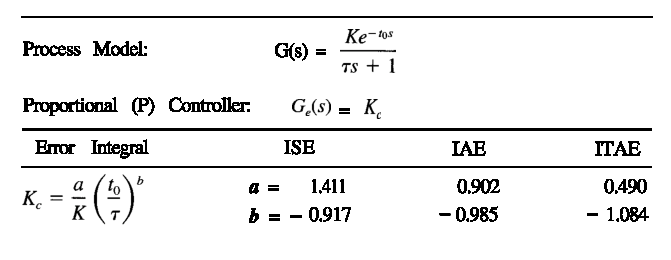
\includegraphics[width=9cm]{images/criteriosOptimosP.eps}
\end{figure}
\end{frame}

\begin{frame}[<+->]\frametitle{Sintonización Óptima para Regulación - Controlador PI}
\begin{figure}
	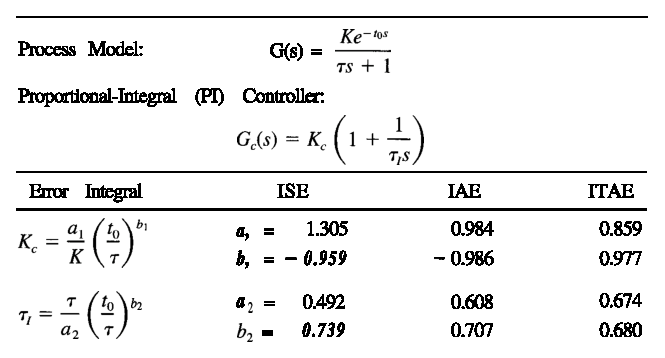
\includegraphics[width=9cm]{images/criteriosOptimosPI.eps}
\end{figure}
\end{frame}

\begin{frame}[<+->]\frametitle{Sintonización Óptima para Regulación - Controlador PID}
\begin{figure}
	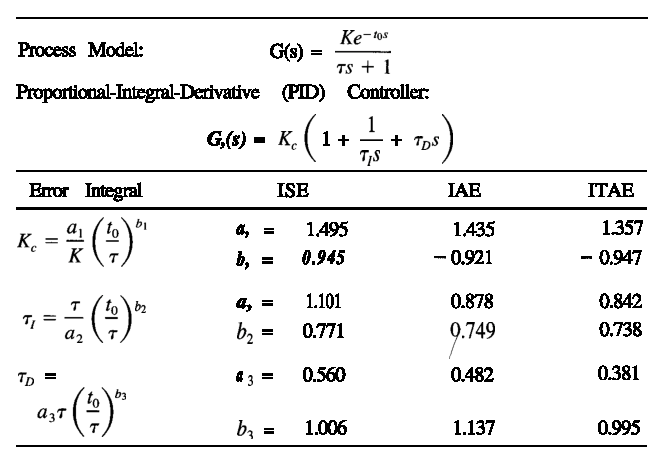
\includegraphics[width=9cm]{images/criteriosOptimosPID.eps}
\end{figure}
\end{frame}

\begin{frame}[<+->]\frametitle{Sintonización Óptima para Servos - Controlador PI}
\begin{figure}
	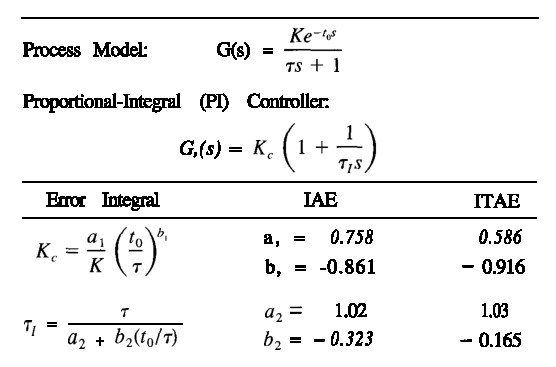
\includegraphics[width=9cm]{images/criteriosOptimosServoPI.eps}
\end{figure}
\end{frame}

\begin{frame}[<+->]\frametitle{Sintonización Óptima para Servos - Controlador PID}
\begin{figure}
	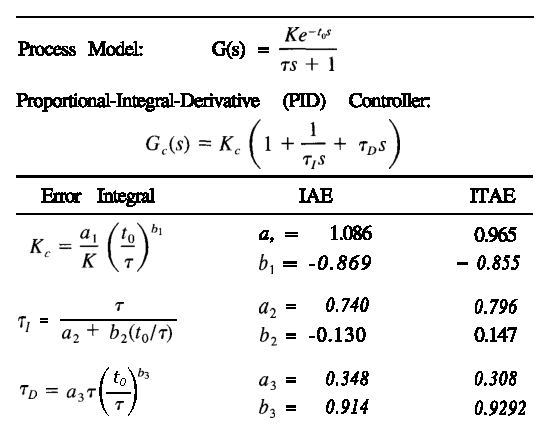
\includegraphics[width=8cm]{images/criteriosOptimosServoPID.eps}
\end{figure}
\end{frame}

\begin{frame}[c]\frametitle{Taller}
	\begin{enumerate}
		\item Considere el sistema de control mostrado en la figura.
		\begin{itemize}
			\item Diseñe un controlador PID usando el método de Ziegler-Nichols.
			\item Determine la respuesta a entrada unitaria y disturbio unitario.
			\item Cuál es el máximo sobrepico y tiempo de establecimiento para la respuesta a entrada unitaria?
		\end{itemize}
		\seti
	\end{enumerate}
	\begin{figure}
		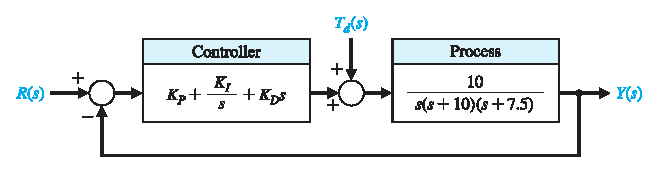
\includegraphics[width=10cm]{images/ejercicio1.eps}
	\end{figure}
\end{frame}

\begin{frame}[c]\frametitle{Taller}
	\begin{enumerate}
		\conti
		\item La siguiente figura muestra la curva de reacción obtenida al aplicar una entrada paso al sistema $G(s) = \frac{1}{(s+1)^4}$.
		\vspace*{-5mm}
		\begin{columns}
		\begin{column}{0.5\textwidth}
		\begin{figure}
			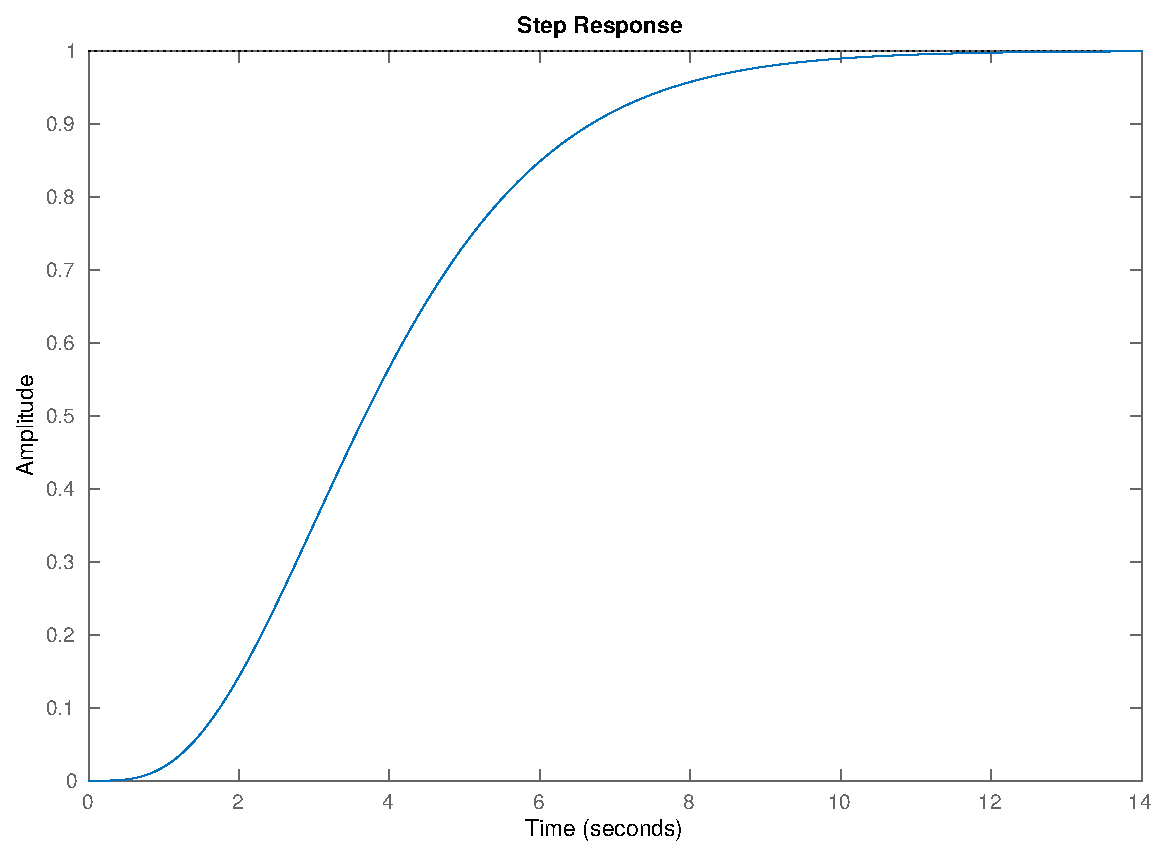
\includegraphics[width=7cm]{images/responseCurve.eps}
		\end{figure}
		\end{column}	
		\begin{column}{0.5\textwidth}
		\begin{itemize}
			\item Encuentre una aproximación de primer orden mas tiempo muerto (FOPDT) para el sistema.
			\item Diseñe un controlador PID usando los métodos de Ziegler-Nichols, Cohen-Coon e ITAE.
			\item Compare los valores de los parámetros obtenidos en cada caso.
			\item Evalue el desempeño de cada controlador ante entrada paso unitario y disturbio paso unitario.
		\end{itemize}
		\end{column}	
		\end{columns}
		\seti
	\end{enumerate}
\end{frame}

\end{document}